\documentclass[12pt, a4paper]{article}
\usepackage[utf8]{inputenc}
\usepackage{graphicx}
\graphicspath{{./Figures/}}
\usepackage[margin=0.5in]{geometry}

\title{Milestone 1}
\author{Jack Byrnes, Raymond Ly}
\date{\today}
\pagenumbering{arabic}

\begin{document}
\maketitle
\tableofcontents
\section{UI and UX design}
We designed our user interface in three steps:
\begin{enumerate}
\item In our competitive analysis, we found strengths and weaknesses in other websites that we would implement and avoid, respectively. 
The weaknesses to avoid were:
\begin{itemize}
\item All pages should be accessible, not hidden in the footer. 
\item The digestion of statistics would be easier if they were presented visually instead of in plain text. 
\item The navigation of the website should be clear (you should be able to get to every relevant page from the navigation bar, not having to follow hyperlinks embedded in other pages. 
\item Any forms should be native not a downloadable PDF. 
\end{itemize}
\item We assessed all of the queries that our user should be able to complete for each level using our website.
\item We came up with a list of elements that would need to be on each page and brainstormed alternative layouts. We then drew a design each for each of the levels, keeping with Nielson's Design Heuristics (Nielson \& Molich 1990) and the requirements of our user (ie what queries they should be able to ask).
\end{enumerate}
Below are the designs of each page with accompanying explanations of design choices, using Nielson's heuristics and personae.
\subsection{Level 1}
\begin{figure}[h]
\centering
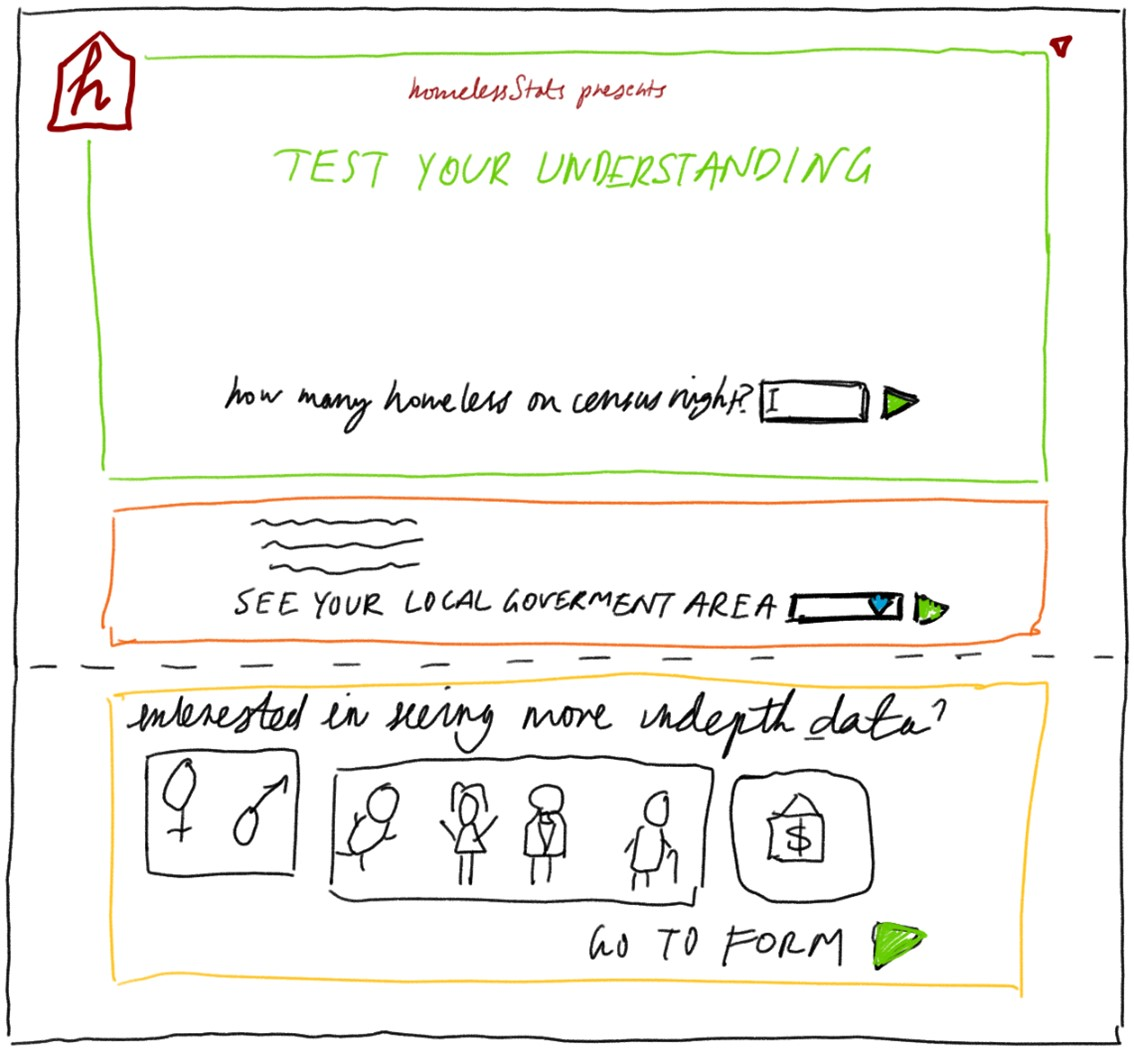
\includegraphics[scale=.8]{LandingPage.jpg} 
\caption{The landing page of the website}
\label{fig:landing}
\end{figure}
\textbf{Landing page} (Figure \ref{fig:landing}) 

Outlined in green, the first feature is a box that the user can click on to get through to the big picture page. Alternatively, the user can type an answer into the text box to the question prompted and click on the arrow button, which will take them to the real value of the question. This method of testing a user's knowledge before showing them data mitigates the Dunning-Kruger effect (Kruger \& Dunning 1999). If there is a disparity in what the user thinks they know about homelessness and what they actually know, this tool will be used to highlight this disparity and thereby inform the user there is information to learn. 

Outlined in orange, the second feature is another box that users can click through to get to the 'shallow glance at homelessness' page. It is populated with text that explains what data they will find on this page. A search bar following text prompts the customer to enter the name of their local government area. Upon submission, they will be taken through to the level 2 results for this LGA. This is especially helpful for Douglas, whose goal is to learn more about homelessness and how he can get involved, specifically in his own community.

These boxes follow Neilson’s Consistency and Standards heuristic, allowing users to intuit that each box serves different functions. The arrows (coloured in green) align with Neilson’s Match Between System and the Real World heuristic, as it is commonly understood that arrows mean forward or to go, catering for users like Douglas. Identified as a strength in StreetSmart Australia’s website were the subtle call-to-actions at any point in the browsing experience, replicated in the arrows. Making our features consistent throughout the page minimises the user’s need to learn how to use the web page, as Neilson’s Recognition or Recall heuristic describes.\\
\begin{figure}[h]
\centering
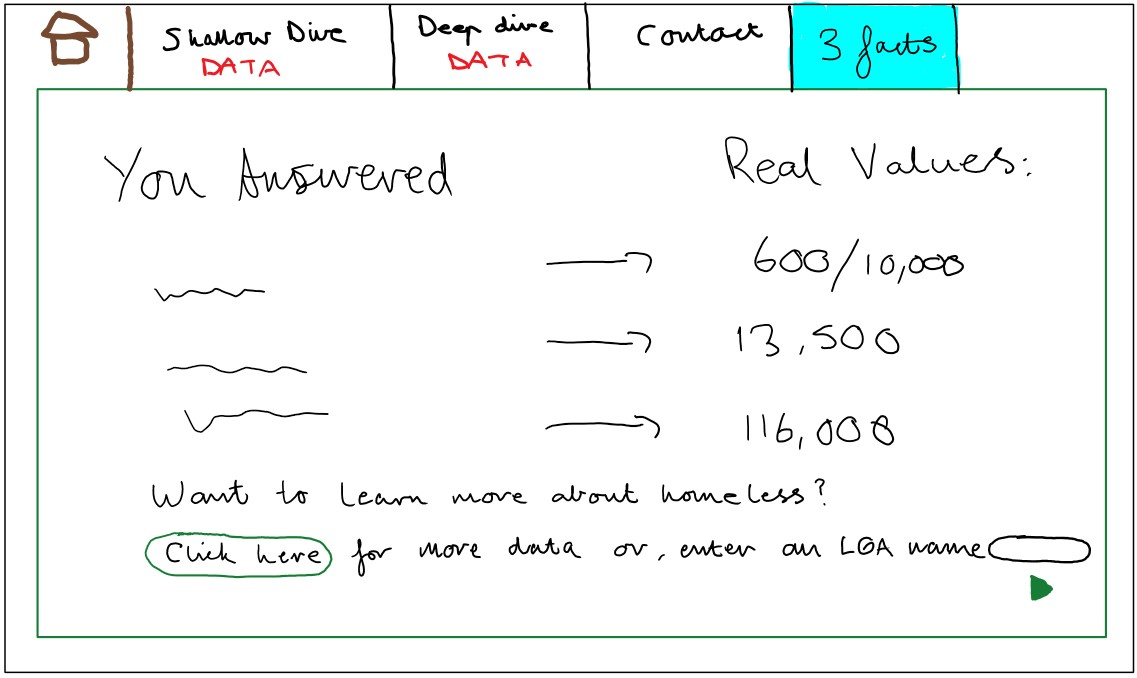
\includegraphics[scale=.6]{3facts.jpg} 
\caption{3 facts page}
\label{fig:facts}
\end{figure}
\textbf{3 facts page} (Figure \ref{fig:facts})\\
Displayed are the users answers and the correct answers. Now that the user has had a little test of their knowledge, they can 'click here' for more knowledge or enter an LGA name. Either option will take them through to the shallow dive data page. If they press 'click here', it will show the information for Australia and it will show the information for the LGA if they entered it. By default all check-boxes will be selected when they first arrive on the page and the toggle will be set to show data on homeless people. We assumed this particular filter setting is more likely than any other one filter setting as it is a total number with no assumptions on what type of gender or age characteristics the user is interested in. 

The filter section allows users to complete queries such as 'show the ranking of LGA's by the amount of homeless women aged 0-40' or 'what is the LGA with the most homeless males?'.

The navigation bar at the top allows the user to get back to the home section or the deep dive data section at any time and shows them which page they are on with a highlight. The navigation bar will be consistent across all pages.

\subsection{Level 2}
\begin{figure}[h]
\centering
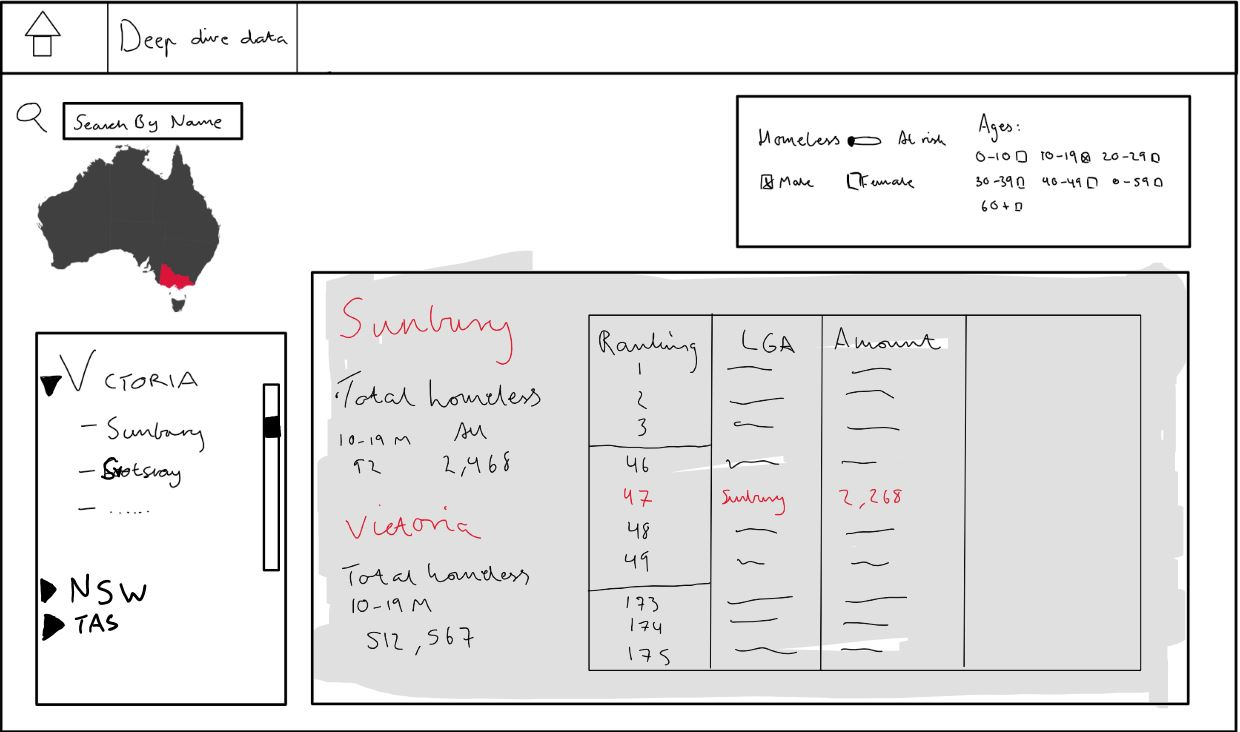
\includegraphics[scale=.6]{level2outer.png} 
\caption{The user input sections of level 2}
\label{fig:2outer}
\end{figure}
\textbf{Level 2 user input} (Figure \ref{fig:2outer}) 

The user is able to select an LGA using the tools on the left of the page. There is an input at the top where they can type in the LGA name and hit 'search'. The two elements beneath the search bar allows the user to select a state and scroll through the list of LGA's in that state. The user can select the state by clicking the are on the map that corresponds to the state or by selecting the state name in the list beneath the map. Having already seen many of the ubiquitous maps of Australia, the user will be able to utilise their real world knowledge while they user our system  (Nielson, Molich 1990). The user can see the aggregate information of Australia by selecting the line outlining the map (Australia-wide will also be an option in the list of states) The user can then scroll through the LGA's in each state by using their touchpad/mouse scroll or the scroller on the side. 

The user can change the filters in the results box by checking each of the options and/or toggling between data on people who are homeless or at risk. 

\begin{figure}[h]
\centering
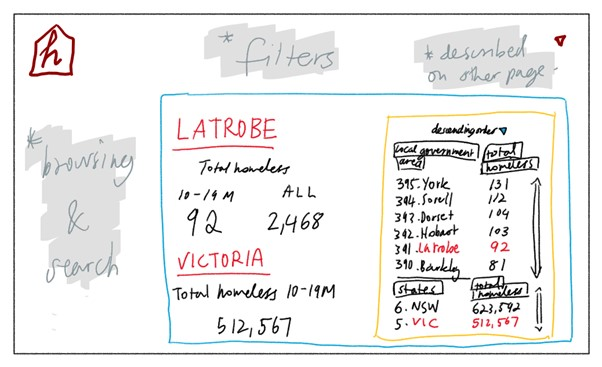
\includegraphics[scale=.9]{level2inner.jpg} 
\caption{The result section of the level 2 page}
\label{fig:2inner}
\end{figure}
\textbf{Level 2 results page} (Figure \ref{fig:2inner}) 

The results of level 2 are encased in the blue box.

The information the user has searched for will be displayed on the left hand side of the results box. If the user came to level 2 without providing an LGA name, the box provides aggregated data of all homeless people in Australia. If the user selects a state by clicking it on the map, the information for that state will be shown. If an LGA is selected, it will appear at the top of the box and the corresponding state below. If the user does input an LGA name on the landing page, their LGA will appear with its state in this format.

Outlined in yellow, the second feature is a ranking table. It displays all LGA's ranked. Immediately, they can see how their LGA or state ranks in terms of total homeless numbers with filters applied. They can also choose to see the list in ascending or descending order.

The chosen local government area and/or state are highlighted through coloured text in the ranking table, meeting Neilson’s Visibility of System Status heuristic, where the user can receive feedback as they switch between different LGAs. 

The ranking feature is separated to the side and is smaller than the main information table. It presents information to users like Douglas, who is only seeking basic information about their community, while also being useful to Lisa, looking for comparative data for her assignment. This describes Neilson’s Flexibility and Efficiency of Use, where the basic user remains uninhibited while the more advanced user can draw some deeper insight.
\subsection{Level 3}
\begin{figure}[h]
\centering
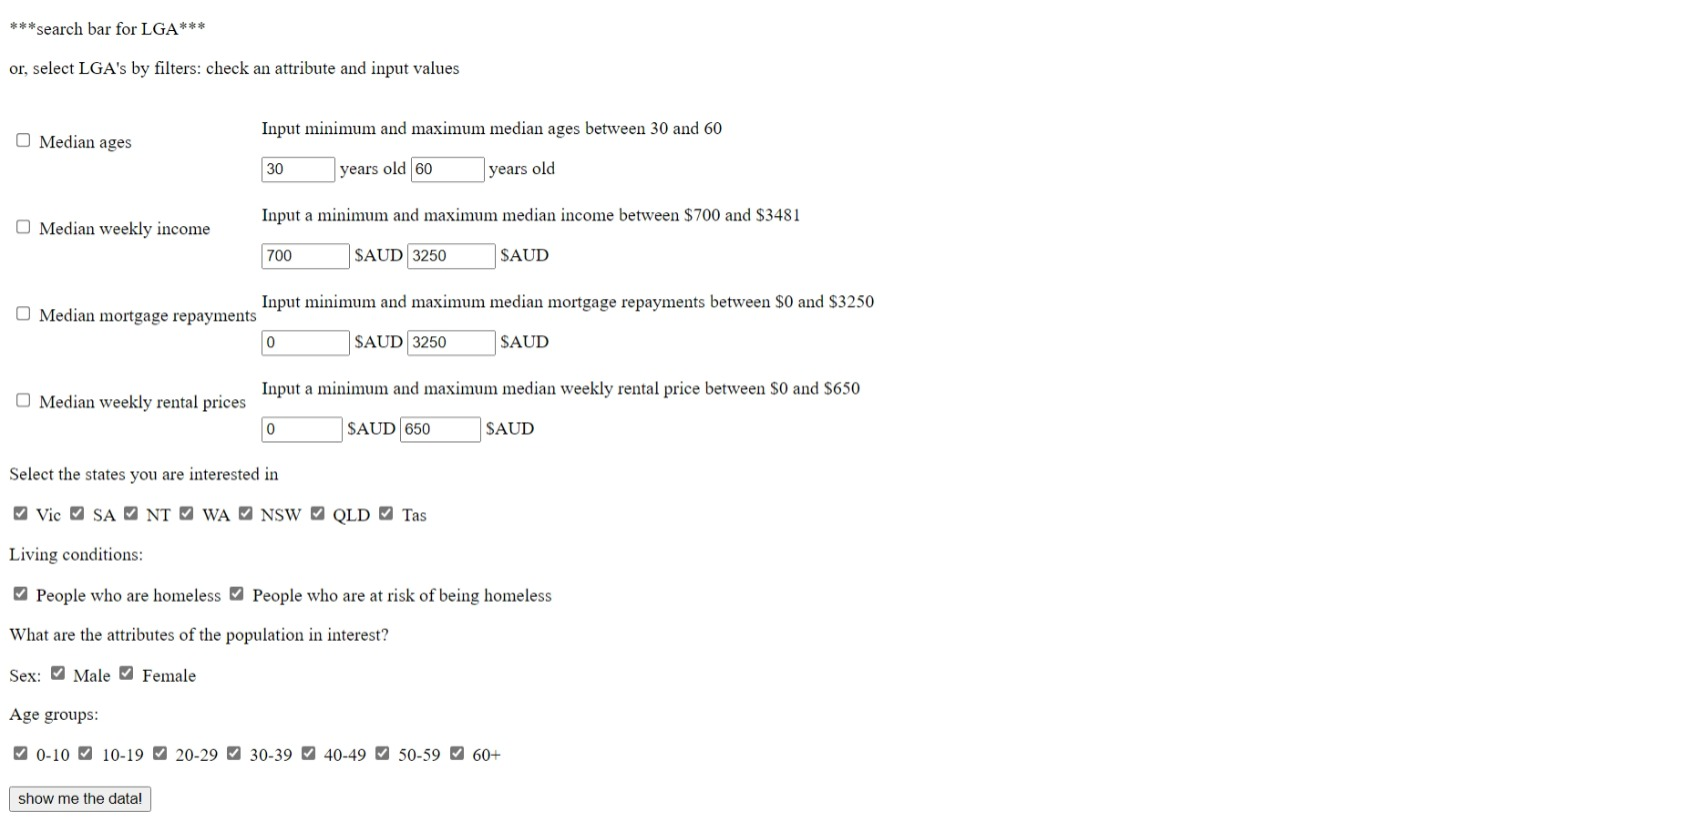
\includegraphics[scale=.9]{level3form.jpeg} 
\caption{The form page of level 3}
\label{fig:3form}
\end{figure}
\textbf{Level 3 form} (Figure\ref{fig:3form})

A user can get any of the required queries answered by first inputting what they would like to see into the form. If a user checks a box relating to the attributes of the LGA they are interested in, that attribute will appear in the table as a column showing the value of that attribute for each LGA. The user can also change the minimum and maximum values of each attribute. LGA's outside of these ranges will be filtered out and not shown on the table. The user can also input a LGA name and the top of the form. The results will be filtered by this text and the only row on the result table will be this LGA. 

If the user wants to see changes in data between 2016 and 2018, they will check both of the 2016 and 2018 check-boxes.  The table will then columns for percentage changes in amount (and only columns for changes, it will not have double the amount of columns as if one year was selected) The 'help' icon next to the 'Years' prompt will inform the user of this function if they click on the icon..
The default selections of the form will be for all states, all ages, all sexes, 2018, Population and none of the LGA attributes (median ages through to median rental prices). This keeps consistency with the second level page (Nielson \& Molich 1990).
 
To test the efficacy of the table, let us look at two complex queries and what form the user would fill out to get the results: 

\textbf{Query one} Enable a user to see if there are any trends of the number of homeless people based on the average weekly income in each LGA. 

The user will check the 'median weekly income' check-box but not change the minimum and maximum. They will then select 'show me the data' and filter the table on the results page by the clicking the sorting arrow in the column header 'weekly income'. They can choose whether the column is sorted by highest to lowest or visa versa by clicking the sorting arrow again. As the user scrolls, they can note trends in the number of homeless people as the weekly income increases or decreases. 

\textbf{Query two} Show if there are any trends of the number of homeless people based on how the percentage change in homeless people (as calculated above) changes as the total population of a LGA changes. 

The user will select the 'Population', 2016 and 2018 check-boxes. The resulting table will show a column for the percentage change in homeless people and for the percentage change in the population for each LGA.

The submit button is labelled 'show me the data' to give insight into what is about to happen next as alternative to 'submit', which can mean multiple things.

The form will save the user input to reduce user recall and improve user control and freedom. If the user made a mistake in entering a value or ticking a box on the form, say ticking 'Vic' instead of 'SA', they will not have to re-enter all of the other information when they realise their mistake while on the results page and return to the form. 

The input boxes do not allow for the user to enter values outside of the range, preventing errors. They also do not require the user to enter the amounts in order, as we can just take the higher amount as the maximum in our query, enhancing user control and freedom.

This level three form is ideal for someone finding in depth information, like Lisa. Lisa may need to find some very specific trends for an assignment on homelessness and not having any expertise with databases makes for a challenging task. If Lisa were to use a program like excel, she would have to perform multiple tasks like summations of columns, column creations and all across multiple files. Our tool allows Lisa to fill out one form, make any necessary changes to the form without losing previous input and export the table as a csv file.

\begin{figure}[h]
\centering
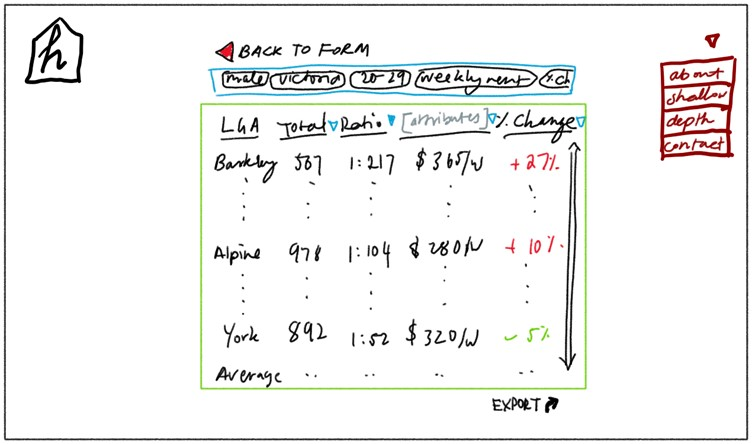
\includegraphics[scale=1]{level3results.jpg} 
\caption{The results page of level 3}
\label{fig:3results}
\end{figure}
\textbf{Level 3 results page} (Figure \ref{fig:3results}) 

This page serves to provide all the information that the user has requested in the form, in the form of a table.

The first feature is the results table, outlined in green. It is displayed in the middle of the page and expands outwards if more information has been requested in the form. The furthest left column will always display LGA name and all of the attributes that the user has selected in the form will be displayed. The red button allows sorting in that column in ascending or descending order. Neilson’s Aesthetic and Minimalist design heuristic is displayed here through the absence any irrelevant information to increase the visibility of the table.

The specifications of the form are displayed in the second feature, outlined in blue. Having the options listed out in this way provides the user with Visibility of System Status, reminding them of the options that they have chosen and allows for review if required. This keeps them informed about exactly what they are seeing in the first feature.

The user can return to the form through the third feature: the back arrow, to edit their specifications to adjust the table. This provides the user with User Control and Freedom, described by Neilson as allowing the user to quickly and simply return in case an error was made.

The table and the specifications can be exported for reference. Lisa, who is doing research on homelessness for her assignment, easily adjusts her preferences and is informed of her specifications until she is satisfied with the table of information and can export it for her own reference.

The user also has the option to return to the home page through the floating home button on the top left, at any point on the website, or navigate to other pages through the navigation drop down bar on the top right, extending on the User Control and Freedom heuristic.

At the bottom of the table is an 'average' row to show the average of each column. This allows users to find answers to queries such as 'What is the homeless ratio of women in LGA's with a weekly income lower than \$500'. After filling out the filters in the form page, they will be able to see the ratio for all of the LGA's in the 'homeless ratio' column in the average row.
\section{Database design}
It was necessary to design a database to allow our website to provide the information the user wants. A user must be able to make relational data queries such as 'show me the homeless ratio in LGA's that have a median weekly income lower than \$500'. We could have all of the information for the LGA's in the one table, with every attribute of that LGA in it's own column (eg. '2016\_homeless\_f\_0\_9' amount of female homeless people who are aged 0-9 in that LGA in 2016). With the current data we have, we would need 45 columns with that database design. 

A table with 45 columns is manageable and if we did not want this project to be scalable, this design would be fine. We want the database to grow as more research is conducted however, and we would be starting to add columns to our database if all the information was in one table. This would require the database to make a copy of the table with the new columns, transfer all of the previous entries and delete the original. The amount of columns in the table would also become more and more unmanageable as more research data becomes available. If we split the data up into multiple tables we avoid this issue and any new data is added as new data entries (rows) without having to do a complete restructure.

To decide how many entities (table) we needed and which attributes (columns) each entity should have, we analysed the data that we have and made an entity diagram (see figure \ref{fig:erdiagram}). The database modelled in the diagram allows for entry of new data without making new attributes. 

\begin{figure}[h]
\centering
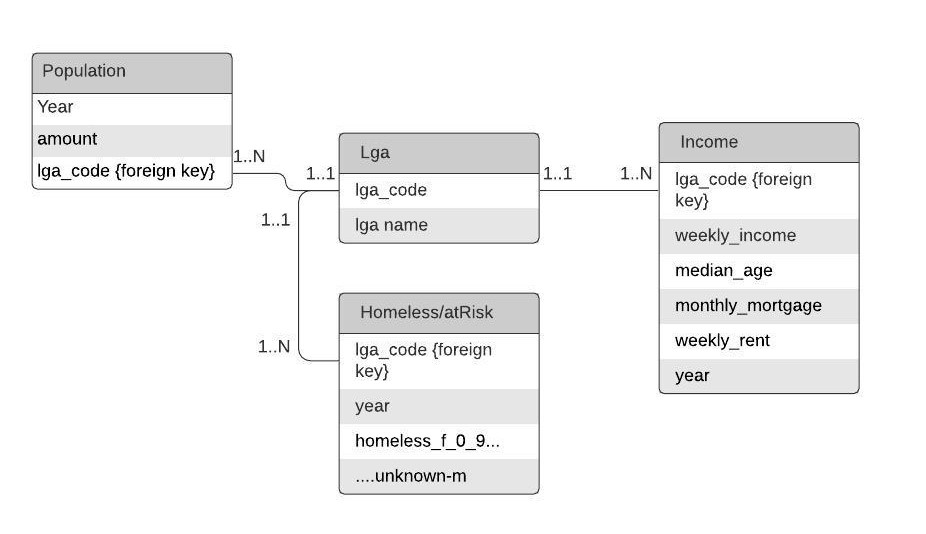
\includegraphics[scale=1]{ERDiagram.jpg} 
\caption{Entity Relationship diagram of the database}
\label{fig:erdiagram}
\end{figure}

\textbf{Relational model}\\
A relational model can be extracted from this diagram:\\
Lga(\underline{lga\_code}, lga name)\\
Population(\underline{lga\_code*, year}, amount)\\
Income(\underline{lga\_code*, year}, weekly\_income, median\_age, monthly\_mortgage, weekly\_rent)\\
Homeless/AtRisk(\underline{lga\_code*, year}, **homeless\_f\_0\_9 ... unknown\_m )\\

\emph{**Note}: The Homeless/AtRisk entity has attributes between the ellipses. Each attribute is an integer amount of the people that meet the conditions stated. For example, the attribute 'homeless\_f\_0\_9' corresponds to people who are homeless, female and between the ages 0 and 9 inclusive. If this attribute were '7', the year attribute '2016' and the lga\_code was the code corresponding to Sunbury, it would mean there were 7 homeless female people aged 0-9 in 2016.\\

The database modelled in figure \ref{fig:erdiagram} enable the website to deliver any information that the user needs. As an example, lets look at how the database would work for a query. To illustrate it's capability we will choose a complex query:

\textbf{Query:} What is the ratio of homeless people against the total population in LGA's where the median weekly income is under \$500. We will assume the user wants the most recent data available and only use data from 2018
These are the steps that are needed in order to answer this query with the data that we have:
\begin{enumerate}
\item Find all of the LGA's that had a median weekly income under \$500 in 2018.
\item Calculate the total number of people in these LGA's who were homeless in 2018.
\item Find the total 2018 population of these LGA's.
\item Divide the result of step 2. by the result of step 3.
\end{enumerate}
In order to answer this query, our database would complete these steps:
\begin{enumerate}
\item Find all of the weekly\_income entries in the Income table that are less than 500 along with the corresponding LGA codes.
\item Find and sum the amounts of all homeless that correspond to these LGA codes in the Homeless/AtRisk table. (all of the attributes that begin with 'homeless' for each LGA.
\item Find and sum the amounts that corresponds to these codes and the year '2018' in the Population table.
\item Divide the result in step 2. by the result in step 3.
\end{enumerate} 

\textbf{Building the database:} 

To build the database, we imported four csv files. Two files resembled two of the tables that we would need in the database: Population and Income. Another two files contained the information that we needed for our Homeless/AtRisk table. All of these files also contained the information needed to create the LGA table: LGA codes with corresponding LGA names. To build our database, we executed the following steps in Sqlite Studio:

\begin{enumerate}
\item Create a database and import all four csv files as tables using the GUI in Sqlite Studio. Resulting in tables: HRA2016, HRA2018, Population and Income.
\item Combine the 2016 and 2018 data on homeless people and people who are at risk of being homeless by executing: 

\hspace*{10mm}%
INSERT INTO [HRA2018]\\
\hspace*{10mm}%
SELECT * FROM [HRA2016];\\
Then renaming HRA2018 to Homeless/AtRisk using the GUI.
\item Creating an LGA table and inserting the LGA code and name columns from the Income table (either Income or Population would have worked here):\\
\hspace*{10mm}%
CREATE TABLE [LGA](\\
\hspace*{10mm}%
lga\_code INT PRIMARY KEY NOT NULL,\\
\hspace*{10mm}%
lga\_name TEXT NOT NULL);\\
\hspace*{10mm}%
INSERT INTO [LGA]\\
\hspace*{10mm}%
SELECT lga\_code, lga\_name FROM Population;
\item Remove the column containing the LGA names from all tables excluding [LGA]. This can be done in a couple of ways, we chose to use the GUI.
\end{enumerate}
To test our database, we wrote SQL scripts corresponding to the queries that are available to the user. Our database will work in conjunction with Java to return the result: 

\textbf{Query:} Show me how the rate of homelessness has changed between 2016 and 2018 in all LGA's compared to population.

A table with these three columns will be able to show the user this information: lga\_name, percentage change in the ratio of homeless people to the total population and the percentage change in population. To see the trend, the user can sort by the third column and then notice the change in numbers in the second column. The user can also easily see any net relationship by referring to the 'total' row at the top of the table, which will show a total change in the homeless ratio and the total change in population across the LGA's. 

To produce this table, our database and Java will work in collaboration (in pseudocode):
\begin{enumerate}
\item Create a new table with the columns detailed above and insert lga\_names from the LGA table into the first column.
\item For each LGA (row), sum all of the columns that refer to homeless people in the Homeless/AtRisk table where the year = 2016.
\item Do the same where the year = 2018.
\item Divide result of 3. by the result of 2 and insert this result into column two of the created table.
\item Divide the 2018 and 2016 populations in the Population table and insert this into the third column.
\end{enumerate}
Each of the columns will match up with an LGA because all of the tables are sorted by lga\_code. 

\textbf{Possible further database features}: \\
Currently we are unsure how we are going to save the level 3 form data for when the user wants to change their query. It may be that we can use html for this but we might have to create a table in the database that stores information on what the user selected in the form. There would be a column for each possible value of every input the user selects. \\

\section{References}

Nielsen, Jakob, and Rolf Molich. “Heuristic Evaluation of User Interfaces.” Proceedings of the SIGCHI Conference on Human Factors in Computing Systems. ACM, 1990. 249–256. Web. \\

Kruger, Justin, and David Dunning. “Unskilled and Unaware of It: How Difficulties in Recognizing One’s Own Incompetence Lead to Inflated Self-Assessments.” Journal of personality and social psychology 77.6 (1999): 1121–1134. Web.
\end{document}
